\chapter{Introduction}
\label{introduction}

%\newpage

\dropcap{E}ver since its introduction in 1983, the Internet has grown to a global communication network used by individuals to interact with others.
Nowadays, numerous companies operate large-scale digital platforms to facilitate on-line interactions between potentially billions of users.
eBay was one of the first platforms that enabled the trustworthy trade of goods between merchants and buyers over the Internet, and is used by millions on a daily basis.
More recently, companies acting in the sharing economy, like Uber and AirBnb, shaped the notion of digital interactions between individuals over the Internet.
These companies facilitate peer-to-peer resource sharing where strangers can share personal resources, like their house or car, in a trustworthy manner.

Most of the on-line applications we use on a daily basis are \emph{centralized}, e.g., managed by a single authority that maintains the required network infrastructure. % facilitated by centralized architectures, often deployed and maintained by a single company.
In particular, when considering a centralized Internet application, there is a single or limited group of servers, responsible for processing all requests submitted by the platform participants, e.g., uploading a video on YouTube or posting a tweet on Twitter.
%Hosting the network infrastructure to facilitate interactions on a global scale requires major investments and platform costs, as exemplified by major companies like Facebook and Google.
On one hand, centralized infrastructures are relatively easy to setup and their performance can be increased by deploying more servers.
On the other hand, even a single software bug or hardware failure could lead to a prolonged unavailability of the entire application.
For example, Facebook experienced a day of downtime in March 2019 due to a server misconfiguration.

In comparison, \emph{decentralized} applications aim to avoid reliance on a single authority.
A decentralized application consists of a network where computers directly communicate and collaborate with each other instead.
One of the most popular decentralized applications is the BitTorrent file transfer protocol, used to share and download torrent files.
In BitTorrent, users directly exchange parts a (potentially large) file with each other over the network, without any requirement for servers that are under the control of a single authority.
Although the global unavailability of a decentralized application is a rare phenomena, they often are more vulnerable to attacks targeted at the network layer, such as the Sybil Attack and the Eclipse Attack.

The introduction of the decentralized Bitcoin cash system in 2008 by Satoshi Nakamoto\footnote{A pseudonym. The real identity behind the pseudonym is (still) unknown.} changed how decentralized applications are built.
Bitcoin is the first electronic cash system with significant adoption, compared to similar proposals, and has gained much interest from both academia and industry.
The system is powered by a blockchain data structure which is a tamper-proof transaction ledger, secured and maintained by users themselves.
Bitcoin is the first system to enable the controlled minting of digital cash without a bank.
Ten years later, blockchain technology is being researched within a large number of domains, including finance, health care, identity and real estate.
In particular, there has been much interest from the open-source developer community to build and deploy decentralized applications powered by blockchain technology.
At the time of writing, there are \todo{X} decentralized applications running only on the Ethereum blockchain.

\begin{figure}[t]
	\centering
	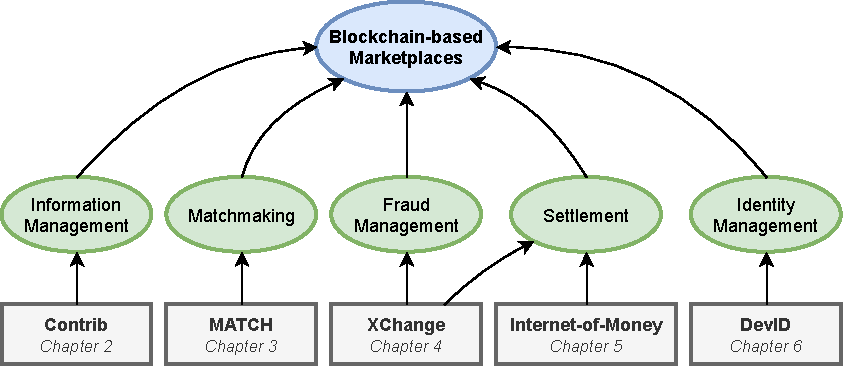
\includegraphics[width=\linewidth]{introduction/assets/thesis_overview}
	\caption{The four mechanisms presented in this work (depicted in grey), in the context of existing technologies (depicted in green).}
	\label{fig:thesis_overview}
\end{figure}

\todo{Introduce thesis here}

%\section{Problem Statement}
%The key issue is that decentralized applications that are using blockchain technology are often not scalable enough.

\section{Research Questions}

The overarching research question of this thesis is as follows:

\emph{How can we improve matchmaking and settlement mechanisms in blockchain-based electronic markets?}\\\\
To answer our research question, we address the following key questions:

\textbf{[RQ1] What is the state-of-the-art in blockchain-based electronic trading and asset exchange?}
To provide an answer to our research question, it is required to build an understanding of state-of-the-art approaches to blockchain-based trading, and their shortcomings.
Even though there is much active research on blockchain-based decentralized exchanges and secure asset trading between heterogeneous blockchain platforms, the field lacks a systematic literature overview, an analysis of open challenges and suggestions for further research.

\textbf{[RQ2] How can we efficiently match market orders without centralized coordinator?}
The predominant approach to order matchmaking in electronic markets is by using a centralized server, owned by the market operator.
This approach, however, enables manipulation by the operator, resulting in an unfair system.
Blockchain-based matchmaking has the potential to address fairness issues but is by far not scalable enough for usage by many marketplaces.
We aim for an efficient matchmaking mechanism with fairness guarantees, not under the control of a single market operator.

\textbf{[RQ3] How can improve settlement durations of (international) payment infrastructures?}
A major problem of current banking systems is that the settlement duration of a payment between two different (international) banks is significant, often in the order of days.
Furthermore, these payments require significant transaction fees to cover back-office costs.
Blockchain technology holds the potential to improve the speed of (international) payment infrastructures, and potentially lead to a reduction of costs and lower transaction fees.

\textbf{[RQ4] How can we exchange assets managed by different blockchains?}
Decentralized exchanges (DEXes) is a new type of decentralized application where digital assets are issued and traded on a blockchain.
Compared to centralized exchanges, DEXes take a non-custodial approach where users manage these assets themselves.
The main issue, however, is that the assets on a specific DEX are locked to a single blockchain; trade between different DEXes is either impossible or slow.
The question is how to address these issues and enable fast asset trading between different exchanges.

\textbf{[RQ5] How can we apply blockchain technology to improve software crowdsourcing markets?}
The engineering of blockchain-based applications such as exchanges is a challenging task and requires engineers with appropriate qualifications.
Crowdsourcing is a relatively new model for software development, where an open call is made for the documentation, design, coding, and testing of software.
Recent research proposes to leverage blockchain technology
Applying accountability and fraud detection could improve the software crowdsourcing process.

\section{Research Methodology}

% add: related research mostly follows a theory-driven approach

Throughout this thesis, we adopt an experimental research methodology to answer our research questions.
We validate our ideas with a software implementation and evaluate them with emulation-based experimentations conducted on our DAS5 compute cluster.
While designing an infrastructure or system, we always aim for a solution that is suitable for adoption and applicable in a real-world environment.

% simplicity?

We believe this experimental research methodology is suitable for two reasons.
First, it allows us to evaluate our ideas in an environment that closely resembles a real-world environment.
Second, it directly leads to a software implementation that can be used by academia or industry.
All developed software artefacts are available on our GitHub repository and contain unit tests to verify functional correctness.

% existing research does X

% but we do Y!

\section{Contributions and Thesis Outline}

After establishing the required background on decentralized applications and distributed ledger technology, Chapter \todo{X} highlights scalability limitations of state-of-the-art blockchain ledgers.
Next, in Chapter \todo{X}, we design, implement and evaluate TrustChain: a scalable blockchain ledger that is based on fraud \emph{detection} instead of fraud \emph{prevention}.
In Chapters \todo{X to Y}, we apply accountability primitives and fraud detection techniques in three well-established domains: financial transactions, two-sided marketplaces, and identity.
Specifically, we make the following contributions in each chapter:\\

\textbf{[Chapter 2] SoK: Electronic Markets in the Age of Blockchain.} (Work in progress)
In this chapter, we answer RQ2 and provide an extensive overview of existing approaches for online trade in the age of blockchain.\\

\todo{Work in progress}\\

\textbf{[Chapter 3] MATCH: Accountable and Generic Matchmaking for Decentralized Applications.}
In this chapter, we partially address RQ4 and focus on matchmaking, the process of bringing market participants together based on individual preferences.
Matchmaking is a cardinal, yet overlooked prerequisite for a fully decentralized exchange.
Although numerous companies have deployed infrastructure for matchmaking, there is currently no solution that can be deployed within different trading domains.
We present MATCH, a middleware for generic order matching.
Since MATCH is agnostic about order specifications, the resulting system is highly flexible and reusable.
In this work, we first present an alternative approach to order matching, named \emph{decentralized matchmaking}.
The main idea is that new orders are disseminated to multiple matchmakers simultaneously and shared between matchmakers.
We then design and implement a novel matching protocol and a middleware with full support for both existing matchmaking paradigms and decentralized matchmaking.
Finally, we extensively evaluate desired system properties of MATCH under a real-world ride-hailing and asset trading workload.
Our main finding is that decentralized matchmaking exhibits superior fault tolerance and load balancing, at the cost of moderately increased bandwidth usage and order completion time.
This chapter is based on the following publication:

\todo{UNDER REVIEW}\\

\textbf{[Chapter 4] XChange: A Scalable Asset Marketplace based on Accountability.}
In this chapter, we answer RQ4 and introduce XChange, an asset marketplace based on accountability guarantees.
There is an increasing need for a generic mechanism to trade assets across isolated platforms, as more industries rely on the digital management of their physical resources using Internet-of-Things devices.
To date, there is no such mechanism without dependency on a trusted third party.
We address this shortcoming and present XChange, a blockchain-based mechanism for generic asset trading.
Unlike existing asset trading marketplaces, we decouple trade management and the actual exchange of assets.
XChange enables the trustworthy trade of \emph{any} digital asset.
We describe a generic trading protocol that establishes trade between individuals and accounts market activity on any distributed ledger.
We prove with a theoretical analysis that the effectiveness of fraud conducted by adversarial parties is limited.
Furthermore, we devise a novel market architecture, composed of all required components for a decentralized asset marketplace.
We implement the XChange mechanism and conduct real-world evaluations.
To account market activity in a tamper-proof manner, we use an existing scalable blockchain ledger, TrustChain.
By deploying XChange on multiple low-resource devices, we show that a full trade can be completed within 500 milliseconds.
To analyze the scalability and bandwidth usage, we conduct further experiments on our compute cluster and deploy up to 500 XChange instances.
Our main finding is that the throughput of XChange, in terms of trades per second, scales linearly with the network size.
This chapter is based on the following publication:

\todo{UNDER REVIEW}\\

\textbf{[Chapter 5] Internet-of-Money: Applying Accountability to Enable Real-time International Money Transfers.}
In this chapter, we answer RQ3 and explore a new stage in the evolution of digital trust, trusting strangers with your money.
We address the challenging problem of giving money to others and relying on them to forward it.
To identity fraud, we account money transfers between interacting strangers.
This work represents a small step towards a generic infrastructure for trust, moving beyond proven, single-vendor platforms like eBay, Uber and AirBnb.
Expanding upon trust relations, we designed, implemented and evaluated an overlay network: \emph{Internet-of-Money}.
Internet-of-Money is capable of real-time money transfers to different banks by routing funds through individuals (\emph{money routers}).
This removes the need for central banks to handle a payment.
Our network reduces traditional payment durations from a day or even a few days in weekends, to mere seconds.
%Internet-of-Money is fully decentralized, privacy-preserving and highly scalable.
With real-world experimentations, we prove that Internet-of-Money enables fast money forwarding.
We show that our overlay network is capable of discovering a majority of available money routers within a minute.
Finally, we demonstrate how profit of cheating routers is limited and that misbehaviour is punished.
This chapter is based on the following publication:

Martijn de Vos and Johan Pouwelse, \enquote{Real-time Money Routing by Trusting Strangers with your Funds}, \emph{IFIP Networking, 2018.}\\

\textbf{[Chapter 6] DevID: Blockchain-based Portfolios for Software Developers.}
In this chapter, we answer RQ5.
Decentralized applications, also known as dApps, are the new paradigm for writing business-critical software.
Recruiting developers with appropriate qualifications and skills for this activity is key, yet challenging.
The main problem is that the portfolio of developers is usually scattered across centralized platforms like GitHub and LinkedIn, and vendor locked.
This can result in an incomplete impression of their capabilities.
We address this problem and introduce \emph{DevID}, a blockchain-based portfolio for developers.
Over time, this portfolio enables developers to build up a trustworthy collection of records that showcase their capabilities and expertise.
They can import data assets from third parties into a unified DevID portfolio, add projects and skills, and receive endorsements.
All portfolio records are stored on a scalable distributed ledger and owned by developers themselves.
The essential idea is to exploit the tamper-proof property of the blockchain while providing durable storage.
To demonstrate the practical value of DevID, we build the competition-based platform, \emph{dAppCoder}, for the development of decentralized applications.
On dAppCoder clients are able to submit their ideas and developers can find work.
dAppCoder utilizes DevID portfolios to match these clients and developers.
We fully implement our ideas and conduct a deployment trial.
Our trial demonstrates that DevID is efficient at storing portfolio records.
This chapter is based on the following publication:

Martijn de Vos, Mitchell Olsthoorn and Johan Pouwelse, \enquote{DevID: Blockchain-based Portfolios for Software Developers}, \emph{IEEE International Conference on Decentralized Applications and Infrastructures (DAPPCON'19)}\\

\textbf{[Chapter 7] Conclusion.} We will end this thesis with the conclusion, a summary of the lessons learned, and suggestions for further work.

%\newpage

%\bibliographystyle{unsrt}
%\bibliography{introduction}